%%%%%%%%%%%%%%%%%%%%%%%%%%%%%%%%%%%%%%%%%%%%%%%%%%%%%%%%%%%%%%%%%%%%%%%%%%%%%%%
\documentclass{article}

\usepackage[french]{babel}
\usepackage[utf8]{inputenc}
\usepackage[T1]{fontenc}
\usepackage{float}

% inclure des images
\usepackage[pdftex]{graphicx}
\usepackage{tikz} 

\title{Rapport d'Algorithmique Avancée \\ Problème de l'arbre de Steiner}

\author{Maxence Perion}
\date{30 Octobre 2022}

\begin{document}
\maketitle 

%\newpage

\tableofcontents
\newpage


% N'hésitez pas à illustrer votre rapport avec des figures.


\section{Le Problème de l'arbre de Steiner}
\subsection{Description et modélisation}
Le problème de l'arbre de Steiner est utilisé notamment pour modéliser le problème de multicast rencontré lors de la diffusion d'un flux de données dans un réseau, où l'on va chercher à optimiser le temps mis par le flux pour atteindre les utilisateurs. \\ \par
\begin{figure}[!h]
	\centerline{ 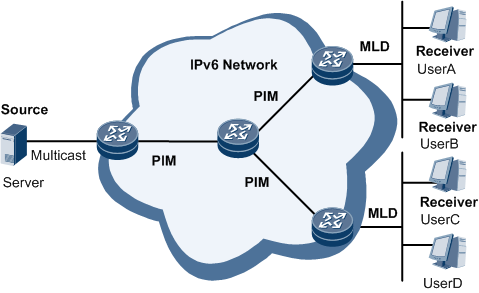
\includegraphics[width=7cm]{images/multicast.png}}
	\caption{Multicast dans un réseau (source: support.huawei.com)}
\end{figure}
Il s'agit donc de trouver les meilleurs chemins (les plus rapides) dans un graphe représentant le réseau. De manière formelle, on peut définir ce problème comme la recherche d'un arbre T couvrant un sous ensemble V' (les noeuds qui doivent être reliés) d' un graphe non orienté G. En tant que problème d'optimisation, nous pouvons le définir comme l'existence ou non d'un tel arbre T couvrant V' tel que le nombre d'arêtes de T soit inférieur à un certain k. Il est possible d'adapter ce problème à un graphe pondéré en recherchant un T dont la somme du poids des arêtes est inférieur à k.

\subsection{Complexité}
Le problème de l'arbre de Steiner est NP complet et nous allons ici en présenter la preuve. 

\subsubsection{Classe NP}
En premier lieu, il faut prouver que ce problème appartient bien à la classe NP, c'est à dire qu'il est possible de vérifier en temps polynomial qu'une solution donnée pour une instance donnée est correcte ou non. \\ \par

Dans notre cas, une solution potentielle est un graphe avec un nombre k' d'arêtes. Il est possible de tester en temps linéaire si k' < k en comptant uniquement le nombre d'arête. De plus, il est également possible de vérifier que le graphe est un arbre en comptant également son nombre de sommets, en temps linéaire également, et en utilisant la formule statuant que le nombre d'arêtes d'un arbre est égal au nombre de sommets moins un. Cette formule peut être démontrée en utilisant la formule d'Euler par exemple. Lors de l'exploration des sommets, il est possible d'en même temps vérifier que le sommet est bien dans G.\\ \par
Pour résumer, si l'on pose n est le nombre de sommets du graphe et m le nombre d'arêtes, il est donc possible de vérifier la solution en au maximum 2 * max(n, m): cela nécessite deux explorations, une des sommets et une des arêtes, et le nombre maximum d'éléments explorés par les deux explorations est majoré par le maximum entre le nombre de sommets et le nombre d'arêtes. La complexité résultante est donc en O(max(n, m)) et ce pour tout graphe.

\subsubsection{Réduction de Set-Cover à Steiner}
Pour prouver que le problème est NP complet, il nous reste à prouver qu'il est NP difficile, c'est à dire qu'il existe une réduction polynomiale (de Karp) de tous les problèmes NP vers le dit problème. Pour cela, nous allons montrer qu'il existe une telle réduction d'un problème déjà démontré comme NP complet vers le problème de Steiner, ce qui est équivalent grâce à la relation de transitivité entre les réductions. \\ \par

Nous prenons comme problème NP complet de départ le problème de Set Cover où le but est, étant donné en ensemble finis S et une famille C de sous-ensembles de S, de couvrir tous les éléments de S avec une sous-famille de C la plus petite possible (ou de taille inférieur à un k donné pour le problème de décision associé). 
\begin{figure}[!h]
	\centerline{ 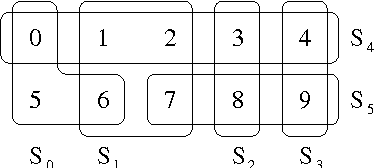
\includegraphics[width=7cm]{images/setcover.png}}
	\caption{Un example d'instance de Set Cover (source: semanticscholar.org, paper: Lazy and Eager Approaches for the Set Cover Problem) \\ Une solution: \{S4, S0, S5\}}
\end{figure}
\\ \par

Partons donc d'une instance de Set Cover avec un certain k, l'ensemble S = \{$V_i$\} pour un certain nombre de $i$, la famille C = \{$S_j$\} pour un certain nombre de $j$ et donc les sous ensembles de S, les $S_j$, sont composés de $V_i$. Nous supposons que tout élément de S apparaît au moins une fois chaque sous famille, autrement dit que chaque $V_i$ est trouvable dans au moins un $S_j$, autrement l'instance n'admettrait pas de solution (et il est possible de le détecter de manière linéaire).\\
L'instance du problème de Steiner associée se compose d'un graphe G construit en ajoutant un sommet dit de départ $S$, un sommet pour chaque ensemble, dit les $S_j$ et un sommet pour chaque élément de S, les $V_i$. L'intuition derrière est que nous cherchons à connecter entre eux les $V_i$ et $S$ ``à travers'' les $S_j$. Ainsi, les arêtes de G vont reliés $S$ à chaque $S_j$ et relier chaque $S_j$ aux $V_i$ qui le composent. L'ensemble V' des sommets à couvrir, dit terminaux, est composés de tous les éléments de S (les $V_i$) ainsi que du sommet de départ $S$. Le nombre d'arête à atteindre dans le problème de Steiner est un k' égal au nombre d'éléments de S plus le k du nombre de famille maximum de Set Cover. En effet, il y aura forcément une arête pour chaque élément (puisqu'il sont terminaux et doivent être tous sélectionnés) ainsi qu'un arête de $S$ pour chaque sous famille sélectionnée.
\\ \par
Cette réduction peut, par exemple, être schématisée comme ceci, avec S =  \{$V_1$, $V_2$, $V_3$, $V_4$, $V_5$\} et C = \{$S_1$, $S_2$, $S_3$\}, où $S_1$=\{$V_1$, $V_2$, $V_3$\}, $S_2$=\{$V_2$, $V_4$, $V_5$\} et $S_3$=\{$V_3$, $V_5$\}:
\vspace{1cm}
\begin{center}
\begin{tikzpicture}[main/.style = {draw, circle}, node distance=2cm] 
\node[main, fill=red] (1) {$S$};

%sets
\node[main] (3) [below of=1]{$S_2$};
\node[main] (2) [left of=3]{$S_1$};
\node[main] (4) [right of=3]{$S_3$};

%elems
\node[main, fill=red] (5) [below left of=2]{$V_1$};
\node[main, fill=red] (6) [right of=5]{$V_2$};
\node[main, fill=red] (7) [right of=6]{$V_3$};
\node[main, fill=red] (8) [right of=7]{$V_4$};
\node[main, fill=red] (9) [right of=8]{$V_5$};

\draw (1) -- (2);
\draw (1) -- (3);
\draw (1) -- (4);

\draw (2) -- (5);
\draw (2) -- (6);
\draw (2) -- (7);
\draw (3) -- (6);
\draw (3) -- (8);
\draw (3) -- (9);
\draw (4) -- (7);
\draw (4) -- (9);
\end{tikzpicture} 
\end{center}
\vspace{1cm}
Cette correspondence entre les deux problèmes est définie de telle sorte qu'une instance de Set Cover est positive si et seulement si l'instance réduite selon la dite réduction est également positive. En quelque sorte, résoudre le problème de Steiner est au moins aussi compliqué que résoudre Set Cover. Ceci conclut donc la preuve de NP complétude. 

\section{Approximation}

\subsection{Algorithme}
Puisque le problème de Steiner est NP Complet, il n'est pas envisageable, pour des raisons de durée d'exécution, de lister toutes les solutions potentielles une à une avec un algorithme dit naïf ou exacte. Il est donc nécessaire d'utiliser un algorithme d'approximation qui va, en échange d'une solution non optimale, donner un résultat rapidement. \\ \par

Pour trouver l'algorithme d'approximation, nous avons remarqué une similitude entre le problème de Steiner et le problème de l'arbre couvrant de poid minimal. En effet,  dans le problème de l'arbre couvrant de poid minimal, l'objectif est de trouver un arbre reliant tous les sommets d'un graphe et dont la somme des arêtes est minimum. Le problème de décision associé cherche à ce que la somme des arêtes soit inférieure à une certaine valeur. \\ 
Puisque le problème de l'arbre couvrant de poid minimal peut être résolu en temps quasi linéaire (E log E) en utilisant l'algorithme de Kruskal par exemple, il est intéressant d'utiliser ce problème pour résoudre celui de Steiner, avec une transformation plus ou moins exacte (à vrai dire elle ne peut pas être exacte sinon Steiner ne serait pas NP Complet). \\ \par

La plus grande différence entre les deux problèmes se situe dans le fait que dans l'arbre couvrant, les sommets à utiliser sont tous ceux du graphe, alors que dans le problème de Steiner il est possible d'utiliser des sommets intermédiaires entre les sommets à relier. Dans notre algorithme d'approximation, nous allons donc chercher à gommer ces sommets intermédiaires en réalisant ce que nous appelons une fermeture métrique, c'est à dire créer un nouveau graphe avec comme sommets les sommets terminaux du problème de Steiner. \\
Étant donné que nous souhaitons les relier entre eux avec un arbre minimal, les arêtes du nouveau graphe vont être ajoutées avec comme pondération le plus court chemin entre les deux sommets dans le graphe de départ, ceci nous permettant de toujours ``considérer'' les sommets intermédiaires. Ces plus courts chemins sont calculés grâce à l'algorithme de Dijkstra. De plus, le nouveau graphe sera complet puisqu'il est possible de relier n'importe quels sommets terminaux et la question est même de savoir quelles combinaisons de chemin entre les noeuds terminaux est la meilleure.\\ \par
 
Grâce à cette version simplifiée, nous pouvons désormais calculer l'arbre couvrant de poid minimal grâce à l'algorithme de Kruskal ou de Prim, en complexité quasi linéaire. Pour finir, il ne nous reste plus qu'à appliquer ce résultat à l'instance du problème de Steiner duquel nous sommes partis. Pour cela, nous nous basons sur le constat que l'arbre couvrant n'a pas sélectionné uniquement des arêtes, mais également la représentation d'un chemin entre les deux sommets de l'arête. Nous allons donc récupérer les chemins correspondants pour notre solution de Steiner, grâce aux plus courts chemins gardés en mémoire et calculés pour faire la fermeture. \\ \par

Il est possible de représenter cet algorithme ainsi:
\vspace{1cm}
\begin{center}
\begin{tikzpicture}[main/.style = {draw, circle},->, node distance=5cm, minimum size=3cm, line width=1pt] 
\node[main,label=above:Instance de Steiner] (1) {Steiner};
\node[main,label=above:Arbre Couvrant minimal] (3) [right of=1]{Graphe complet};
\node[main] (2) [below of=3]{Arbre Couvrant minimal};
\node[main] (4) [left of=2]{Solution de Steiner};


\draw(1) -- (3) node [midway, above=-1cm] {Dijkstra};
\draw (3) -- (2) node [midway, right] {Kruskal};
\draw (2) -- (4) node [midway, below=0.5cm] {Déployement des pcc};

\end{tikzpicture} 
\end{center}
\vspace{1cm}

La complexité de cet algorithme d'approximation dépend surtout de la résolution de l'arbre couvrant minimum, qui s'effectue en temps quasi linéaire. En plus de ça, il faut aussi prendre en compte le calcul des plus courts chemins entre les sommets terminaux, qui s'effectue en temps polynomial puisqu'il s'agit de l'algorithme de Dijkstra. Pour finir, le ``dépliage'' des arêtes s'effectue en temps linéaire puisqu'il n'y a pas de nouveau calcul. En conclusion, on peut supposer que cet algorithme d'approximation est de complexité polynomiale.

\subsection{Rapport d'approximation}
Puisque nous savons qu'un résultat de l'algorithme d'approximation n'est pas forcément optimal, il est intéressant de se demander à quel point il peut être inexacte. \\ 
Pour construire et démontrer notre rapport d'approximation, nous cherchons d'abord à construire une structure, dont on connait la taille, qui majorera toujours notre solution. Notons $T^*$ l'arbre optimal (purement hypothétique). Nous allons d'abord dupliquer les arêtes de $T^*$ afin d'obtenir un cycle eulérien noté $C$. On a donc comme score que $C$ = $2T^*$ puisque toutes les arêtes ont été doublées. On va ensuite ``appliquer'' plus ou moins l'algorithme sur cette nouvelle structure pour montrer que le résultat sera toujours meilleur. On parcours donc les terminaux de $C$ pour construire un autre graphe $C'$ en appliquant les plus courts chemins, on a donc $C'$ $\leq$ $C$. \\
$C'$ ainsi construit correspond à un cycle dans le graphe complet associé $K$, que l'on note $C''$. Puisque $C''$ est un cycle, la suppression d'une de ses arêtes construit un arbre $A''$. On a donc $A''$ $\leq$ $C''$ puisque $A''$ à une arête en moins. De plus, $C''$ = $C'$ puisqu'ils correspondent et on avait $C'$ $\leq$ $C$, ce qui nous donne $A''$ $\leq$ $C$ et $C$ = $2T^*$. Pour finir, puisque l'algorithme de Kruskal nous donne un arbre couvrant $A^*$ minimal, on a  $A^*$ $\leq$ $A''$. Pour résumer, $A^*$  est notre solution et on a  $T^*$ $\leq$ $A^*$ $\leq$ $2T^*$. Notre algorithme est donc une 2-approximation.

\section{Métaheuristique}
Une autre façon de trouver des solutions (approchées) à un problème NP Complet en temps raisonnable est d'utiliser des métaheuristiques. Nous avons choisis d'en implémenter deux différents: le recuit simulé et un algorithme dit génétique.

\subsection{Recuit Simulé}
Le recuit simulé est un algorithme inspiré de phénomènes physiques en métallurgie, où l'on va chercher à parfois baisser la température, parfois la relever. L'objectif de cette algorithme est purement de trouver un minimum dans une fonction donnée. Puisque cet algorithme n'est pas exacte, il est néamons possible de rester bloquer dans un minimum local et non global. \\ \par 

La trame générale de l'algorithme est précédée de la donnée de différents paramètres tels que l'instance du problème à traiter (le graphe et les terminaux dans le cas du problème de Steiner), une température initiale et une température de fin. Il est également possible de trouver un paramètre lié à la méthode de mise à jour de la température choisie, qui peut être exponentielle, linéaire, par palier, ... \\ 
L'algorithme débute avec un état (une solution pontentielle) aléatoire ou défini, qui va correspondre à la meilleure solution jusqu'alors. On va ensuite, pour un nombre d'itérations définis, générer un nouvel état à partir du meilleur état courant grâce à la fonction de voisinage (qui est à définir) et calculer une probabilité de le considérer comme le nouveau meilleur état. Si la fonction d'évaluation (qui est elle aussi à définir) donne un meilleur score à cette nouvelle solution, alors on va définir la propabilité de le choisir comme meilleur à 1, c'est à dire à tous les coups. Sinon, on lui laisse quand même une chance en lui donnant une probabilité égale à l'exponentielle de l'opposé de la différence entre le score de la nouvelle solution moins le score de la meilleur solution, divisé par la température actuelle. \\
Dans tous les cas, on finit par mettre à jour la température actuelle selon la méthode choisie. \\ \par 

\begin{figure}[!h]
	\centerline{ 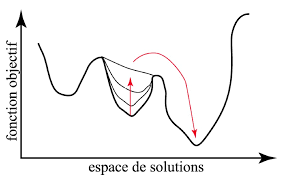
\includegraphics[width=7cm]{images/recuitsimule.png}}
	\caption{Représentation imagée de la recherche de minimum dans la fonction d'évaluation (source: gerad.ca) }
\end{figure}

Pour notre implémentation, nous avons choisit de mettre à jour la température de manière exponentielle et un état complètement aléatoire comme point de départ. Conçernant les températures, nous avons choisit de les calculer automatiquement afin d'obtenir un algorithme valable pour toutes les instances du problème sans avoir besoin de changer les paramètres à la main. \\
Pour cela, nous résolvons l'équation du calcul de la probabilité afin d'obtenir environ 60\% au départ et environ 0.1\% à la fin. Le problème qui s'est posé est qu'il était nécessaire d'évaluer la différence attendue entre la meilleure solution et un de ses voisins au début et à la fin. Pour cela, nous avons trouvé qu'il était pertinent de considérer cette différence comme étant celle dans le pire des cas au début et celle dans le meilleur des cas à la fin, selon la fonction d'évaluation. En effet, il est probable qu'au début de l'algorithme la solution ne soit pas du tout adapté et se fasse fortement punir (le pire des cas: grande différence de score) alors qu'à la fin, il est plutôt probable que les solutions soit toutes adaptées et que la fonction d'évaluation donne des scores très proche (le meilleur des cas: infime différence de score).

\subsection{Algorithme génétique}
L'algorithme génétique est quant à lui inspiré de la biologie et de la sélection naturelle. En effet, en partant d'une population de p éléments, le but va être de générer e enfants et de sélectionner les p meilleurs selon la fonction d'évaluation. Les nombres e et p sont donnés comme paramètres de l'algorithme et vont potentiellement dépendre de l'instance du problème à traiter. Lors de la sélection il est tout à fait envisageable de considérer à la fois les parents et les enfants, ou bien uniquement les enfants. \\ \par

La génération des enfants est également empruntée à la biologie: cette fonction va prendre deux parents et retourner un enfant en combinant les gènes des deux parents. Les dits gènes ne sont autre que la représentation de la solution en question; qui va donc être mixée avec une autre dans le but d'en générer une meilleure. Dans notre cas, nous avons choisis de générer un point aléatoire entre 0 et le nombre de gènes, appelé crossover, qui va marquer la séparation entre la provenance des gènes. En d'autres termes, tous les gènes de l'enfant avant le point crossover proviendront d'un parent et tous ceux après de l'autre. De manière analogue à la biologie, la survenance d'une mutation sur ces gènes lors de la reproduction est possible avec une probabilité donnée en paramètre de l'algorithme. Dans notre cas, nous avons choisis, si une mutation survient, de sélectionner un gène aléatoire et de l'échanger.

\begin{figure}[!h]
	\centerline{ 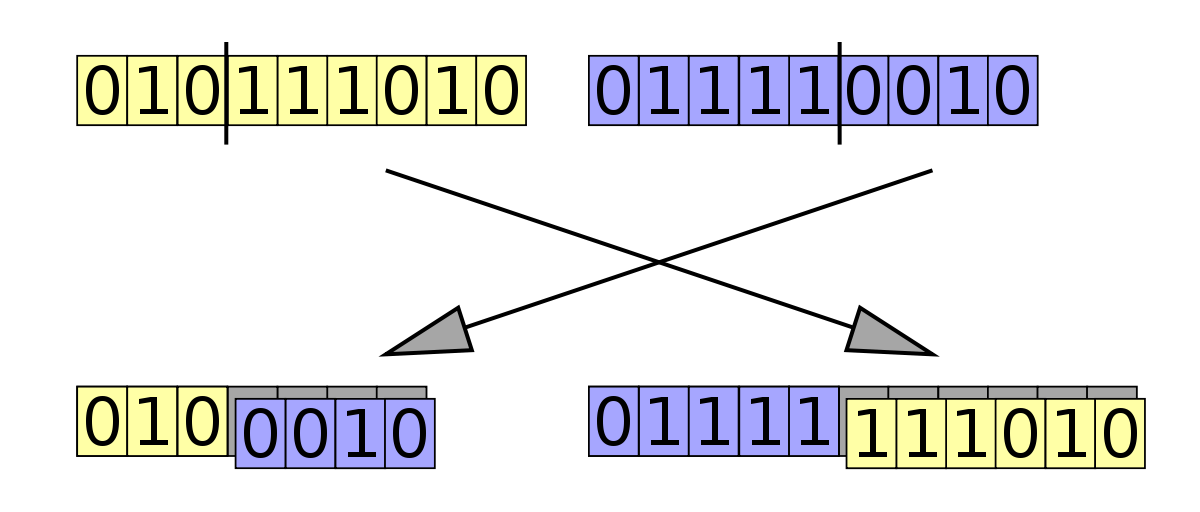
\includegraphics[width=7cm]{images/algogenetique.png}}
	\caption{Représentation imagée de la génération de nouveaux individus selon leurs gènes (source: vikidia.fr) }
\end{figure}

\subsection{Représentation d'une solution}
Préalablement à l'implémentation de ces deux algorithmes, il nous a fallu définir comment nous allions représenter des états ou des solutions potentielles. Puisque le problème se situe dans un graphe et qu'un graphe est définis par ses sommets et ses arêtes, deux choix se sont rapidement imposés à nous: un état représente une liste d'arêtes ou bien une liste de sommets (faire un mix des deux paraît trop vague et l'espace des solutions trop grand). Dans les deux, on associe une valeur booléenne à chaque objet pour indiquer si l'objet est sélectionné ou non. \\ \par

Après avoir expérimenté avec la liste des arêtes et obtenu de mauvais résultats (les graphes n'étaient pas des arbres), nous avons décidé de nous concentrer sur la liste des sommets, avec laquelle nous obtenions de bien meilleurs résultats. Ce choix vient également avec un petit sacrifice en temps puisque pour évaluer une solution, nous devons passer par le calcul de l'arbre couvrant minimal (algorithme de Kruskal encore une fois) entre les différents sommets sélectionnés. Ceci n'était pas nécessaire lors de la sélection des arêtes car nous avions déjà les arêtes du graphe et nous pouvions donc inférer les sommets en question. Cependant, ce sacrifice reste acceptable car il s'effectue en temps quasi linéaire.

\subsection{Voisinage entre solutions}
Les deux algorithmes (et les metaheuristiques en général) requièrent de pouvoir passer d'une solution à une autre, différente. Cette opération est réalisée grâce à la fonction de voisinage, dont la conception est à la responsabilité du programmeur puisqu'elle dépend de la représentation des solutions et donc du problème à résoudre. \\ \par

Dans notre cas, nous nous sommes contenté d'échanger une valeur booléenne aléatoire par sa négation. Cette opération est basique mais permet d'avoir des solutions relativement proches tout en aillant la possibilité de générer n'importe quel élément de l'espace des solutions.

\subsection{Fonction d'évaluation d'une solution}
Afin de quantifier à quel point une solution est proche de ce que nous cherchons (la solution optimale), nous devons mettre en place une fonction d'évaluation. Puisque nous cherchons à minimiser la taille de l'arbre et donc le nombre d'arêtes, la base de notre fonction d'évaluation est ainsi le nombre d'arête de la solution. Ainsi, plus la solution est éloignée de celle optimale, plus son score est élevé. \\
Ensuite, l'arbre doit par définition et pour répondre au problème, être connexe. Nous comptons donc le nombre de composantes connexes et appliquons une pénalité multipliée par le nombre de composantes connexes moins 1 puisque nous autorisons une composante. Pour finir, il est possible qu'un noeud terminal ne soit pas dans le graphe solution, ce qui ne réponds pas au problème posé. Nous pénalisons donc également pour chaque terminal non présent. \\ \par

Si la pénalité en cas d'erreur était trop faible il serait possible que l'algorithme minimise le graphe de façon incorrecte. Par exemple si cette pénalité est de 1, alors il est possible de se retrouver dans une situation où il vaut mieux avoir 2 composantes connexes si la distance qui les séparent est de plus d'une arête. De la même façon, il serait possible d'obtenir un score égal au nombre de terminaux si l'on ne sélectionne aucun sommet. Pour pallier ce problème, nous avons définit la pénalité au nombre d'arête du graphe de départ. Ainsi, une solution défectueuse aura forcément un score plus élevé que n'importe quelle solution conforme, la plus mauvaise soit-elle. Pour finir, nous avons choisis de pénalisé à chaque fois chaque erreur le nombre de fois où elle est présente afin de pouvoir réduire graduellement les erreurs et de diriger une solution très défectueuse de plus en plus vers une solution conforme. Ainsi, il n'y a pas de ``sauts'' dans les évaluations et le développement s'effectue de manière continue.


\section{Résultats expérimentaux}
Nous allons désormais présenter les divers expérimentations que nous avons réalisé afin de justifier nos choix. Les graphes obtenus sont les résultats de 10 exécutions de l'algorithme selon les paramètres en question, la courbe étant la moyenne des résultats obtenus à chaque étape et la zone bleutée représente l'intervalle de confiance obtenu avec la formule classique: $moyenne +/- 2*math.sqrt(variance)/ math.sqrt(n)$. La variance est également obtenu de manière classique en prenant la somme des carrés de la différence entre une valeur et la moyenne. \\
L'axe des abscisses des graphiques représente le nombre d'itérations (ou générations) et l'axe des ordonnées représente les scores donnés par la fonction d'évaluation. Par soucis de temps, nous avons effectués nos tests uniquement sur deux instances du probème: B02 et B04.

\subsection{Recuit Simulé}

\subsubsection{Mise à jour de la température}
Étant donné que nous avons choisis de calculer automatique les températures de départ et d'arrivée en fonction du graphe, choisir une méthode de mise à jour linéaire de la température aurait été contradictoire puisque le nombre d'itération aurait donc été réglable à la main et il aurait fallu le changer selon chaque graphe. Nous avons donc opté pour une mise à jour exponentielle: $T = learnRate * T$, où learnRate est notre paramètre quantifiant la vitesse de descente de la température et nous allons ici justifier son choix. Le but de ces premières expériences est donc de trouver ce $learnRate$ de manière à ce que la solution la meilleure possible ai le temps d'être trouvée sans non plus provoquer une exécution trop longue. \\ \par

Nous démarrons notre expérience en prenant les valeurs 0.9, 0.99 et 0.999 et comparons les résultats obtenus:

\begin{figure}[H]
	\centerline{ 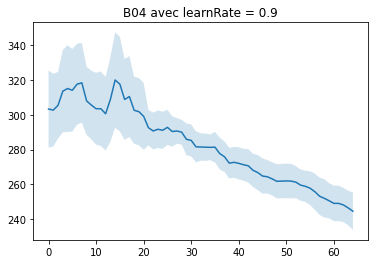
\includegraphics[width=7cm]{images/B04learnrate09.png} 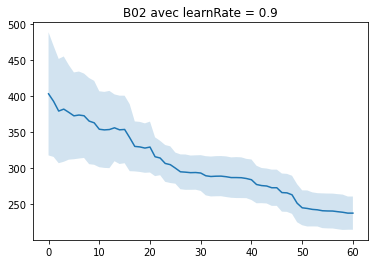
\includegraphics[width=7cm]{images/B02learnrate09.png} } 
\end{figure}
\begin{figure}[H]
	\centerline{ 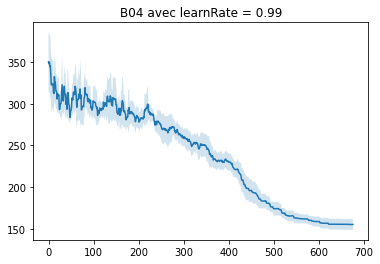
\includegraphics[width=7cm]{images/B04learnrate099.png} 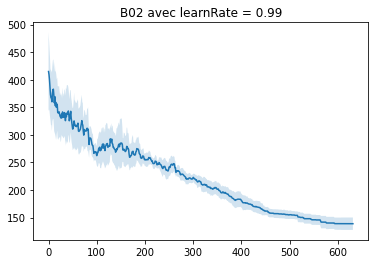
\includegraphics[width=7cm]{images/B02learnrate099.png} } 
\end{figure}
\begin{figure}[H]
	\centerline{ 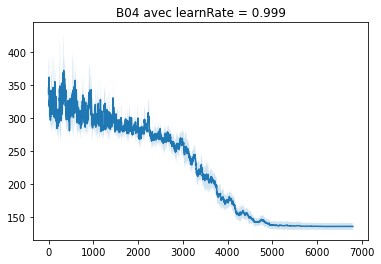
\includegraphics[width=7cm]{images/B04learnrate0999.png} 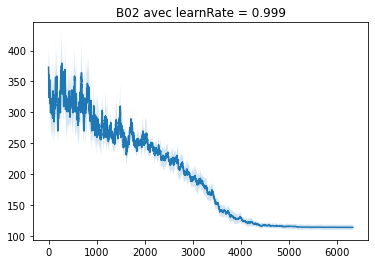
\includegraphics[width=7cm]{images/B02learnrate0999.png} } 
\end{figure}

Nous pouvons constater qu'il est encore possible d'obtenir de meilleurs résultats avec 0.9 et 0.99 puisque la courbe continue de descendre. Pour $learnRate=0.999$, il y a trop de valeurs et la visualisation de la courbe devient compliquée vers la fin. Nous allons donc effectuer un zoom en tronquant à partir de la 3000e itération.

\begin{figure}[H]
	\centerline{ 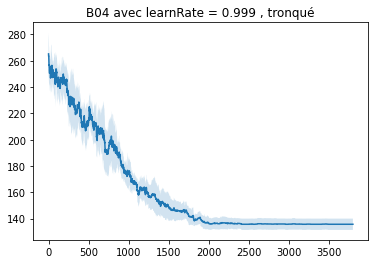
\includegraphics[width=7cm]{images/B04learnrate0999t.png} 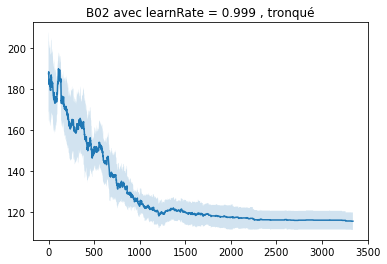
\includegraphics[width=7cm]{images/B02learnrate0999t.png} } 
\end{figure}

Nous pouvons maintenant voir que le score décroit jusqu'à la 5000e génération (3000+2000) pour finir par se stabiliser et atteindre son minimum: 0.999 est donc un bon compromis entre vitesse et précision.

\subsubsection{Températures de départ et d'arrivée}
Nous allons désormais nous intéressé à l'influence des températures de départ et d'arrivée sur la qualité du résultat. Puisque nous les calculons automatiquement, cela revient à s'intéresser à la probabilité attendue au début et celle attendue à la fin. Dans ce type d'algorithme, un constat général est que nous souhaitons une probabilité de changer de meilleur état grand au début puis minime à la fin. Dans ce fait, nous allons nous pencher sur les paires de probabilités suivantes: (0.7, 0.2), (0.6, 0.1), (0.5, 0.01) et (0.9, 0):

\begin{figure}[H]
	\centerline{ 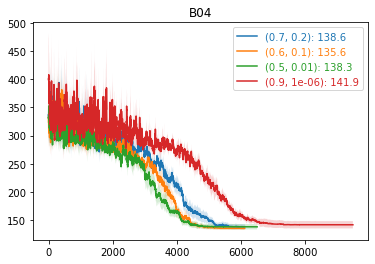
\includegraphics[width=7cm]{images/B04temp.png} 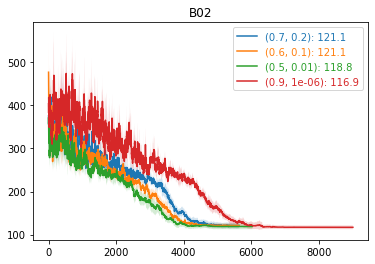
\includegraphics[width=7cm]{images/B02temp.png} } 
\end{figure}

Nous pouvons voir qu'avec toutes les températures, on finit par arriver environ au même résultat. Cependant, ces expériences nous permettent également de constater qu'en plus du coefficient de croissance (learnRate), les températures de départ et d'arrivée ont une influence sur le nombre d'itérations, ce qui est logique. Ainsi, nous pouvons voir que la courbe verte est généralement tout le temps en dessous des autres et c'est donc la paire de probabilités que nous choisissons.

\subsection{Algorithme Génétique}

\subsubsection{Nombre d'individu et d'enfants}
Les paramètres les ayant en premier une incidence directe sur la qualité de la solution obtenu par l'algorithme génétique sont le nombre d'individu par génération et le nombre d'enfants, c'est à dire la population. Non seulement ces deux paramètres doivent être adaptés au problème, mais ils doivent également être cohérents entre eux: ils marchent par paire. Nous allons en quelque sorte premièrement rechercher la recette gagnante puis ensuite chercher combien de fois nous devons l'appliquer. \\ \par

Nous allons donc ici fixer un nombre de générations (50) et un taux de mutation (0.2) et comparer différentes combinaisons de valeurs pour le nombre d'individus et d'enfants de chaque génération. Le but va être de regarder quelle combinaison obtient le meilleur score. Étant donné que générer plus d'enfants revient à considérer plus de solutions à chaque fois, nous allons également fixer le nombre d'enfants par génération à 10 et faire varier le nombre d'individu que l'on garde (parmi les meilleurs). 

\begin{figure}[H]
	\centerline{ 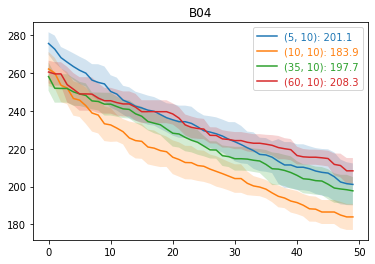
\includegraphics[width=7cm]{images/B04pop.png} 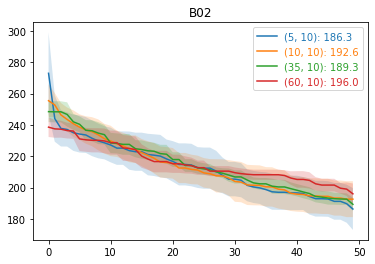
\includegraphics[width=7cm]{images/B02pop.png} } 
\end{figure}

Nous pouvons remarquer sur ces graphiques que plus on garde un nombre restreint de meilleurs éléments, meilleur finit par être le score à la fin, même si ce n'est pas forcément le cas au début.  Cependant, il faut également veiller à en conserver suffisament. Nous pouvons interpréter cela comme la contrainte de garder un ``bon fil conducteur'' dans l'espace des solutions, tout en le laissant assez vague pour éviter les minimums locaux.\\ 
Pour finir, remarquons que cette expérience n'est pas très précise étant donné que tous les intervalles de confiance se chevauchent.

\subsubsection{Mutation}
Pour pouvoir parcourir suffisament l'espace des solutions, nous pouvons expérimenter sur la probabilité de mutations en ayant fixé le nombre de générations et la population.

\begin{figure}[H]
	\centerline{ 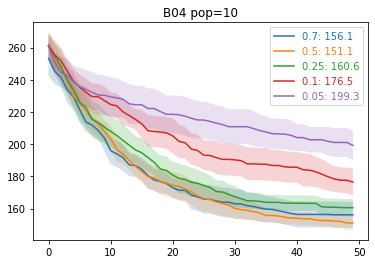
\includegraphics[width=7cm]{images/B04mut10.png} 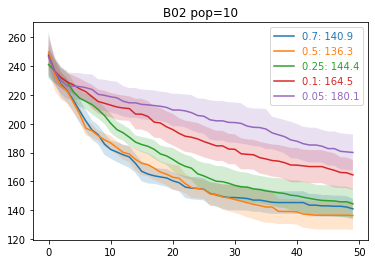
\includegraphics[width=7cm]{images/B02mut10.png} } 
\end{figure}

\begin{figure}[H]
	\centerline{ 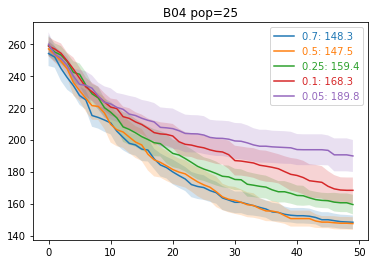
\includegraphics[width=7cm]{images/B04mut25.png} 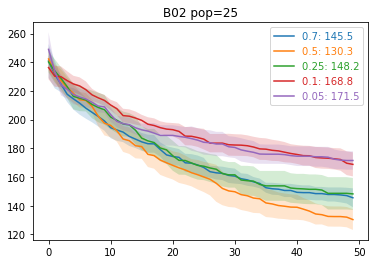
\includegraphics[width=7cm]{images/B02mut25.png} } 
\end{figure}

Nous pouvons donc voir qu'indépendament du nombre d'individus gardés en stock et de manière contre intuitive, la meilleur solution est atteinte avec une probabilité de moitié de muter. Nous pouvons également confirmer ici que l'algorithme donne de meilleurs résultats avec un plus grand nombre d'individus dans la population.

\subsubsection{Nombre de générations}
Après avoir affiné notre recette en dressant des relations entre les paramètres, nous allons maintenant voir jusqu'à quand il est nécessaire de la laisser mijoter. Pour cela, nous sélectionnons comme paramètres 25 individus, 30 enfants et une mutation de 0,5 et cherchons à partir de combien de générations le résultat stagne.

\begin{figure}[H]
	\centerline{ 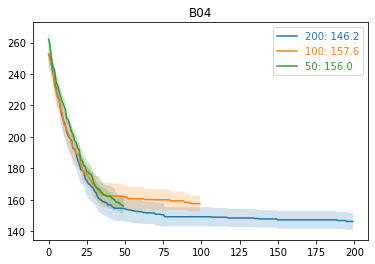
\includegraphics[width=7cm]{images/B04gen.png} 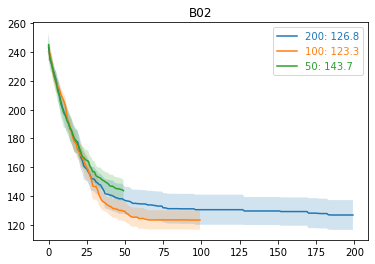
\includegraphics[width=7cm]{images/B02gen.png} } 
\end{figure}

Nous pouvons conclure des ces graphiques qu'un nombre adéquate de générations se situe à 150 environ. Cependant, il faut remarquer que cela dépend fortement de la taille du graphe.

\subsection{Performances}
Le but de ces algorithmes était de résoudre de manière inexacte un problème. Puisque nous avons à notre disposition un algorithme approché et que nous connaissons le résultat optimal attendu sur ces graphes, nous allons comparer le tout afin de nous donner une idée des performances des différents algorithmes. Pour cela, nous allons uniquement considérer la solution finale de chaque algorithme (et non plus son évolution au fil du temps). Cette fois ci, nous allons lancer chaque algorithme 50 fois.

\begin{figure}[H]
	\centerline{ 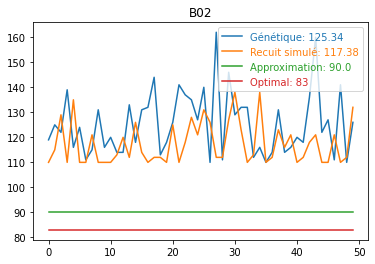
\includegraphics[width=7cm]{images/B02perf.png} 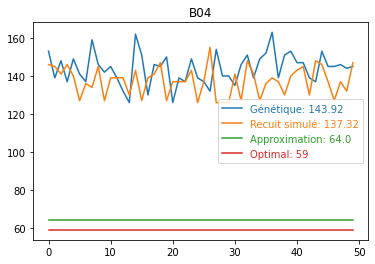
\includegraphics[width=7cm]{images/B04perf.png}} 
\end{figure}

Nous pouvons voir que l'approximation produit un résultat très proche de celui optimal et que les heuristiques que nous avons créée produisent de moins bon résultats, qui sont toujours environ un peu moins de deux fois plus que l'optimal. Pour finir, nous pouvons voir que les deux méthodes produisent dans notre cas des résultats de score similaires.

\section{Conclusion}
Pour conclure, nous avons implémenté différents algorithmes afin de résoudre le problème de Steiner. Ces algorithmes produisent des solutions qui ne sont pas forcément optimales afin de pallier au temps nécessaire pour résoudre ce problème NP Complet. En menant des expérimentations rigoureuses (graphiques, intervalles de confiance, ...) nous avons pu adapter les paramètres de nos algorithmes et confirmer/infirmer nos choix théoriques.

\end{document}

